
\begin{figure}[ht]
    \centering
    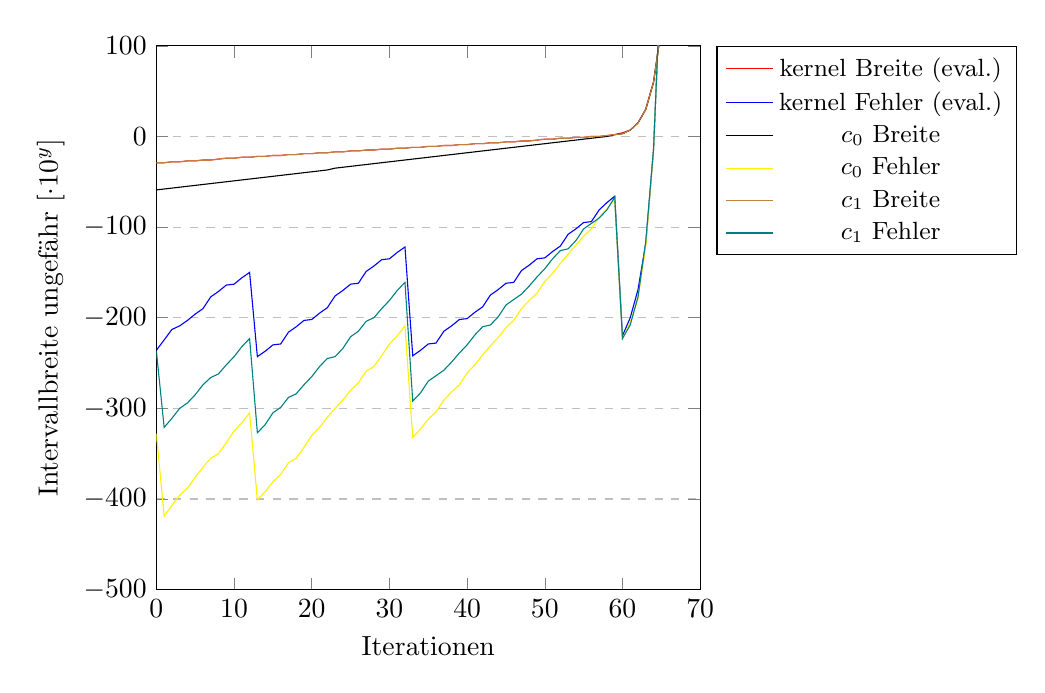
\begin{tikzpicture}
    \begin{axis}[
        width=0.7\textwidth,
        height=0.7\textwidth,
        xlabel={Iterationen},
        ylabel={Intervallbreite ungefähr $[\cdot 10^y ]$},
        legend pos=north west,
        xmin=0,xmax=70,
        ymax=100,ymin=-500,
        ymajorgrids=true,
        grid style=dashed,
        legend pos=outer north east,
        cycle list name=color list
    ]
    
    \addplot
        coordinates {
 (0,-29)
 (1,-29)
 (2,-28)
 (3,-28)
 (4,-27)
 (5,-27)
 (6,-26)
 (7,-26)
 (8,-25)
 (9,-24)
 (10,-24)
 (11,-23)
 (12,-23)
 (13,-22)
 (14,-22)
 (15,-21)
 (16,-21)
 (17,-20)
 (18,-20)
 (19,-19)
 (20,-19)
 (21,-18)
 (22,-18)
 (23,-17)
 (24,-17)
 (25,-16)
 (26,-16)
 (27,-15)
 (28,-15)
 (29,-14)
 (30,-14)
 (31,-13)
 (32,-13)
 (33,-12)
 (34,-12)
 (35,-11)
 (36,-11)
 (37,-10)
 (38,-10)
 (39,-9)
 (40,-9)
 (41,-8)
 (42,-8)
 (43,-7)
 (44,-7)
 (45,-6)
 (46,-6)
 (47,-5)
 (48,-5)
 (49,-4)
 (50,-3)
 (51,-3)
 (52,-2)
 (53,-2)
 (54,-1)
 (55,-1)
 (56,0)
 (57,0)
 (58,01)
 (59,02)
 (60,04)
 (61,07)
 (62,015)
 (63,030)
 (64,060)
 (65,0120)
        };
        \addlegendentry{\small{kernel Breite (eval.)}}
    
    \addplot
        coordinates {
  (0,-236)
 (2,-213)
 (3,-209)
 (4,-203)
 (5,-196)
 (6,-190)
 (7,-177)
 (8,-171)
 (9,-164)
 (10,-163)
 (11,-156)
 (12,-150)
 (13,-243)
 (14,-237)
 (15,-230)
 (16,-229)
 (17,-216)
 (18,-210)
 (19,-203)
 (20,-202)
 (21,-195)
 (22,-189)
 (23,-176)
 (24,-170)
 (25,-163)
 (26,-162)
 (27,-149)
 (28,-143)
 (29,-136)
 (30,-135)
 (31,-128)
 (32,-122)
 (33,-242)
 (34,-236)
 (35,-229)
 (36,-228)
 (37,-215)
 (38,-209)
 (39,-202)
 (40,-201)
 (41,-194)
 (42,-188)
 (43,-175)
 (44,-169)
 (45,-162)
 (46,-161)
 (47,-148)
 (48,-142)
 (49,-135)
 (50,-134)
 (51,-127)
 (52,-121)
 (53,-108)
 (54,-102)
 (55,-95)
 (56,-94)
 (57,-81)
 (58,-73)
 (59,-66)
 (60,-220)
 (61,-200)
 (62,-169)
 (63,-118)
 (64,-14)
 (65,191)
        };
        \addlegendentry{\small{kernel Fehler (eval.)}}
       
    
    \addplot
        coordinates {
 (0,-59)
 (1,-58)
 (2,-57)
 (3,-56)
 (4,-55)
 (5,-54)
 (6,-53)
 (7,-52)
 (8,-51)
 (9,-50)
 (10,-49)
 (11,-48)
 (12,-47)
 (13,-46)
 (14,-45)
 (15,-44)
 (16,-43)
 (17,-42)
 (18,-41)
 (19,-40)
 (20,-39)
 (21,-38)
 (22,-37)
 (23,-35)
 (24,-34)
 (25,-33)
 (26,-32)
 (27,-31)
 (28,-30)
 (29,-29)
 (30,-28)
 (31,-27)
 (32,-26)
 (33,-25)
 (34,-24)
 (35,-23)
 (36,-22)
 (37,-21)
 (38,-20)
 (39,-19)
 (40,-18)
 (41,-17)
 (42,-16)
 (43,-15)
 (44,-14)
 (45,-13)
 (46,-12)
 (47,-11)
 (48,-10)
 (49,-9)
 (50,-8)
 (51,-7)
 (52,-6)
 (53,-5)
 (54,-4)
 (55,-3)
 (56,-2)
 (57,-1)
 (58,0)
 (59,02)
 (60,03)
 (61,07)
 (62,015)
 (63,030)
 (64,060)
 (65,0119)
        };
        \addlegendentry{\small{$c_0$ Breite}}
        
    \addplot
        coordinates {
  (0,-328)
 (1,-419)
 (2,-407)
 (3,-396)
 (4,-388)
 (5,-376)
 (6,-365)
 (7,-355)
 (8,-350)
 (9,-338)
 (10,-325)
 (11,-316)
 (12,-305)
 (13,-401)
 (14,-392)
 (15,-381)
 (16,-373)
 (17,-360)
 (18,-355)
 (19,-343)
 (20,-330)
 (21,-321)
 (22,-310)
 (23,-300)
 (24,-291)
 (25,-280)
 (26,-272)
 (27,-259)
 (28,-254)
 (29,-242)
 (30,-229)
 (31,-220)
 (32,-209)
 (33,-332)
 (34,-323)
 (35,-312)
 (36,-304)
 (37,-291)
 (38,-282)
 (39,-274)
 (40,-261)
 (41,-252)
 (42,-241)
 (43,-231)
 (44,-222)
 (45,-211)
 (46,-203)
 (47,-190)
 (48,-181)
 (49,-173)
 (50,-160)
 (51,-151)
 (52,-140)
 (53,-130)
 (54,-120)
 (55,-110)
 (56,-102)
 (57,-89)
 (58,-80)
 (59,-69)
 (60,-223)
 (61,-205)
 (62,-179)
 (63,-121)
 (64,-15)
 (65,191)
        };
        \addlegendentry{\small{$c_0$ Fehler}}
    
        \addplot
        coordinates {
 (0,-29)
 (1,-29)
 (2,-28)
 (3,-28)
 (4,-27)
 (5,-27)
 (6,-26)
 (7,-26)
 (8,-25)
 (9,-24)
 (10,-24)
 (11,-23)
 (12,-23)
 (13,-22)
 (14,-22)
 (15,-21)
 (16,-21)
 (17,-20)
 (18,-20)
 (19,-19)
 (20,-19)
 (21,-18)
 (22,-18)
 (23,-17)
 (24,-17)
 (25,-16)
 (26,-16)
 (27,-15)
 (28,-15)
 (29,-14)
 (30,-14)
 (31,-13)
 (32,-13)
 (33,-12)
 (34,-12)
 (35,-11)
 (36,-11)
 (37,-10)
 (38,-10)
 (39,-9)
 (40,-9)
 (41,-8)
 (42,-8)
 (43,-7)
 (44,-7)
 (45,-6)
 (46,-6)
 (47,-5)
 (48,-5)
 (49,-4)
 (50,-3)
 (51,-3)
 (52,-2)
 (53,-2)
 (54,-1)
 (55,-1)
 (56,0)
 (57,0)
 (58,01)
 (59,02)
 (60,03)
 (61,07)
 (62,015)
 (63,030)
 (64,060)
 (65,0119)
        };
        \addlegendentry{\small{$c_1$ Breite}}
    
        \addplot
        coordinates {
   (0,-237)
 (1,-321)
 (2,-311)
 (3,-300)
 (4,-294)
 (5,-285)
 (6,-274)
 (7,-266)
 (8,-262)
 (9,-252)
 (10,-243)
 (11,-232)
 (12,-223)
 (13,-327)
 (14,-318)
 (15,-305)
 (16,-299)
 (17,-288)
 (18,-284)
 (19,-274)
 (20,-265)
 (21,-254)
 (22,-245)
 (23,-243)
 (24,-234)
 (25,-221)
 (26,-215)
 (27,-204)
 (28,-200)
 (29,-190)
 (30,-181)
 (31,-170)
 (32,-161)
 (33,-292)
 (34,-283)
 (35,-270)
 (36,-264)
 (37,-258)
 (38,-249)
 (39,-239)
 (40,-230)
 (41,-219)
 (42,-210)
 (43,-208)
 (44,-199)
 (45,-186)
 (46,-180)
 (47,-174)
 (48,-165)
 (49,-155)
 (50,-146)
 (51,-135)
 (52,-126)
 (53,-124)
 (54,-115)
 (55,-102)
 (56,-96)
 (57,-90)
 (58,-81)
 (59,-67)
 (60,-223)
 (61,-208)
 (62,-177)
 (63,-116)
 (64,-14)
 (65,190)

        };
        \addlegendentry{\small{$c_1$ Fehler}}
    
    
    \end{axis}
    \end{tikzpicture}
    \caption{$x_0 = [0.5 \pm 0] + [0 \pm \varepsilon] \cdot \lambda ,\ \lambda \in [1 \pm 0]$}
    \label{fig:tm5}
\end{figure}